\chapter{Opis budowy robota}
\section{Wstęp}
Rozdział przedstawia zadania postawione przed robotem, zostaną zrealizowane w ramach pracy inżynierskiej. Zawarte jest w nim także porównanie podobnych konstrukcji, których elementy zostały przeanalizowane i wybrane do budowy konstrukcji. Zawiera też opis użytych modułów wraz z argumentacją wyboru.
\section{Zadania do realizacji przez robota}
\begin{itemize}
    \item \textbf{Przetworzenie informacji o położeniu względem wyznaczonej ścieżki}
    Na podstawie pomiaru uzyskanego z czujników odbiciowych znajdujących się nad zakreśloną trasą wprowadzana jest korekta trajektorii.
    \item \textbf{Obserwacja otoczenia}
    Na podstawie pomiaru uzyskanego z czujników ultradźwiękowych znajdujących się na czole robota określenie odległości od przeszkody i próba ominięcia jej.
    \item \textbf{Analiza informacji o położeniu wału silnika}
    Zapisywanie kroków przebytych przez każde z kół po zjechaniu z linii.
    \item \textbf{Wyznaczenie położenia robota}
    Wyznaczenie odległości przebytej od punktu porzucenia trasy w skutek napotkania przeszkody.
    \item \textbf{Próba powrotu na ścieżkę }
    Poprzez zachowanie bliskiej odległości od przeszkody próba powrotu na ścieżkę.
    \item \textbf{Podjęcie decyzji o ewentualnym niepowodzeniu zadania}
    W momencie osiągnięcia położenia początkowego, bądź oddalenia się zbytnio od linii podjęcie decyzji o zatrzymaniu platformy.
\end{itemize}

\section{Podobne konstrukcje}
Robot jest połączeniem dwóch klasycznych konstrukcji, robota podążającego po linii oraz robota omijającego przeszkody.

Roboty podążające po linii często wykorzystują czujniki własnej konstrukcji zbudowane z użyciem transoptorów. Takie podejście pozwala dostosować kształt wiązki czujników do kształtu maszyny, jednakże wymaga własnego projektu modułu. Często takie rozwiązania odczytują bezpośrednio napięcie z fotodiody, przez co konieczne jest wykorzystanie przetwornika ADC \cite{line_czujnik}. Problem ten można rozwiązać przez dodanie kondensatorów, a następnie pomiar czasu ich rozładowania na portach I/O procesora, tak jak to zostało wykonane w projekcie. 

Dobrym rozwiązaniem do obserwacji otoczenia jest zastosowanie czujników odległości na czole pojazdu  \cite{line_sharp}. Jednakże ze względu na szerokość wiązki fali czołowej zastosowanie czujników ultradźwiękowych pozwala uzyskać większy kąt pomiaru, a także mniejszą wrażliwość na chropowate powierzchnie. Robot spełniający podobne zadania, jednakże bez funkcji omijania przeszkody wyposażony w czujnik ultradźwiękowy może pełnić funkcje robota przemysłowego jako wózek AGV, wykorzystywany do transportu towarów w magazynie \cite{AGV}.

Dość innowacyjnym sposobem jest zastosowanie silników krokowych do napędu robota mobilnego. Takie rozwiązanie pozwala na dokładne sterowanie w otwartej pętli sterowania, tym samym na bieżąco jest śledzona pozycja robota.\cite{kurosz} Jednak wiąże się to jednocześnie z ograniczeniem prędkości robota w porównaniu do użycia innych silników prądu stałego \cite{Tadeo}. W przedstawionej pracy nie zależy na uzyskaniu prędkości przejazdu, a precyzji sterowania, by możliwie jak najdokładniej określić położenie robota względem linii.

\section{Opis zastosowanych modułów}
Podrozdział zawiera opis zastosowanych czujników wraz z uzasadnieniem wyboru w ramach projektu. Wybory te są wynikiem analizy konstrukcji mających spełniać zbliżone zadania. Tym samym sprawdzana jest prawidłowość doboru elementów.
\subsection{Opis konstrukcji typu Line Follower -- czujniki linii}
Celem konstrukcji jest podążanie po wyznaczonej trasie. Podczas zawodów robotycznych jest wykorzystywana czarna linia na kontrastowym białym podłożu, co pozwala robotowi na jednoznaczne określenie trasy poprzez użycie czujników odbiciowych składających się z par: dioda  IR razem z fototranzystorem. Dodatkowo poprzez włączenie w obwód kondensatorów, pozwala na cyfrowy odczyt wartości poprzez pomiar czasu rozładowania danego kondensatora. W projekcie został użyty gotowy moduł składający się z ośmiu par takich czujników.
\begin{figure}[H]
\centering
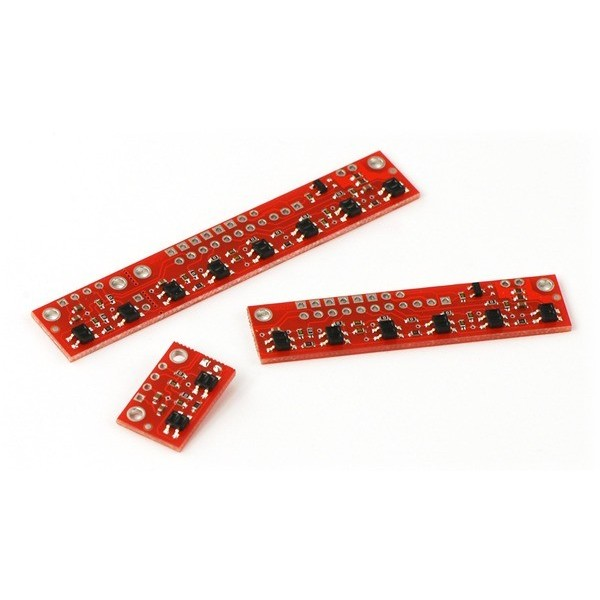
\includegraphics[width=0.5\textwidth]{inzynierku/img/listwa.jpg}
\caption{\label{fig:czujnik_odbiciowy}Listwa z czujnikami odbiciowymi QTR-8RC - cyfrowa.}
\end{figure}

\subsection{Opis konstrukcji typu Micromouse -- czujniki odległości}
Jest to robot, którego głównym zadaniem jest rozpoznawanie odległości do ściany. W przypadku tego projektu odległości do przeszkody. W celu realizacji owego zadania można wykorzystać jeden z wielu typów czujników odległości. Porównanie typów czujników zostało zawarte w Tablicy~\ref{tab:odleglosc}. W projekcie został użyty czujnik ultradźwiękowy.

\begin{table}[H]
\centering
\begin{tabular}{c|c|c}
\textbf{Rodzaj czujnika}        & \textbf{Zalety}           & \textbf{Wady}                     \\ \hline
\multirow{4}{*}{Ultradźwiękowe} & Kąt: \textless 15°        & Martwa strefa 2 cm                \\
                                & Dokładność: 0,3 cm + 1 \% & Czuły na chropowatość powierzchni \\
                                & Napięcie zasilania: 5 V   &                                   \\
                                & Pobór prądu 3 mA          &                                   \\ \hline
\multirow{2}{*}{Typu SHARP}     & Prostota implementacji    & Zasięg od 10 cm                   \\
                                &                           & Pobór prądu 33 mA                 \\ \hline
\multirow{2}{*}{Laserowe}       & Brak martwej strefy       & Czujnik cyfrowy                   \\
                                &                           & Punktowe działanie               
\end{tabular}
\caption{\label{tab:odleglosc}Zalety i wady danych typów czujników w zastosowaniu budowy robota podążającego po linii z funkcja omijania przeszkód. \cite{czujniki, sharp, laser}} 
\end{table}
\begin{figure}[H]
\centering
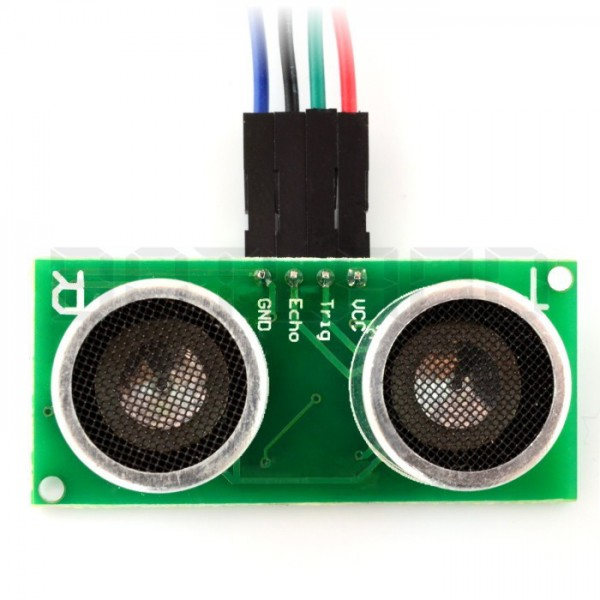
\includegraphics[width=0.5\textwidth]{inzynierku/img/czujnik.jpg}
\caption{\label{fig:czujnik_ultradzwiekowy}Ultradźwiękowy czujnik odległości US-015 2-400cm.}
\end{figure}

\subsection{Dobór silników}
Biorąc pod uwagę brak odpowiedzi z otoczenia na temat położenia robota względem przeszkody w otoczeniu należy pobierać dane o jego przybliżonym położeniu bezpośrednio z silników. Ze względu na rozmiar pracy odrzuca się silniki prądu zmiennego. Jednym z możliwych rozwiązań jest zastosowanie modelarskich silników prądu stałego, jednakże to rozwiązanie wymaga zastosowanie enkoderów do określenia przybliżonego położenia robota. Z tego powodu sensownym jest użycie silników krokowych, za pomocą których przybliżone położenie robota otrzymujemy już zadając ruch. Duża waga, ponad $220g$ każdego z silników pozwala zwiększyć siłę grawitacji $F_g=mg$, co pozytywnie wpływa na docisk kół do podłoża przez co zmniejszony jest efekt poślizgu. Celem platformy nie jest pokonanie trasy w jak najkrótszym czasie, prze co waga nie wpływa negatywnie na właściwości robota. W projekcie użyte są dwa silniki krokowe, posiadają one następujące właściwości:
\begin{itemize}
    \item rozdzielczość $1,8^\circ$;
    \item napięcie znamionowe wynoszące $12,0 V$;
    \item pobór prądu na cewkę $0,4 A$;
    \item moment trzymający $0,25 Nm$.
\end{itemize}
\begin{figure}[H]
\centering
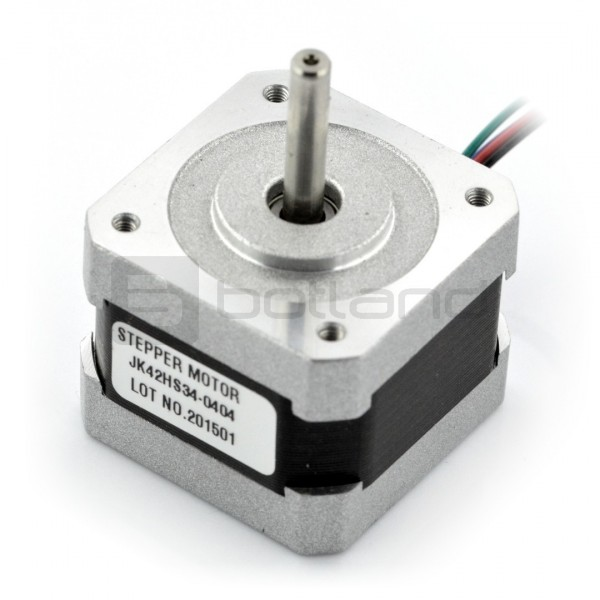
\includegraphics[width=0.5\textwidth]{inzynierku/img/silnik.jpg}
\caption{\label{fig:silnik_krokowy}Silnik krokowy JK42HS34-0404 200 kroków.}
\end{figure}

\subsection{Dobór sterowników silników}
Ze względu na problematyczność sterowania silnikami oraz prądy płynące przez silniki w projekcie użyto gotowych modłów do sterowania silnikiem. Dobierając takich moduł należy zwrócić uwagę na napięcie znamionowe silników, oraz zapotrzebowanie prądowe. Sterownik silnika należy dobrać z zapasem. Zastosowanie owego modułu pozwala na sterowanie silnikiem jedynie za pomocą dwóch wyjść z płytki uruchomieniowej. Na sterownik podawane są sygnały:
\begin{itemize}
    \item kroku;
    \item kierunku obrotu.
\end{itemize}
\begin{figure}[H]
\centering
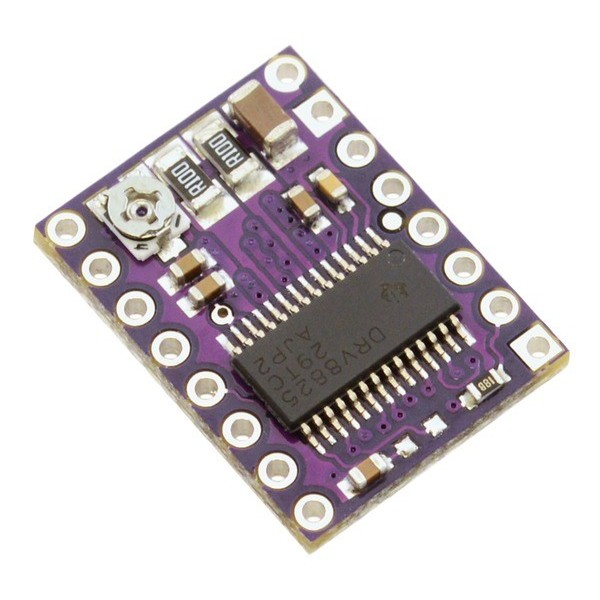
\includegraphics[width=0.5\textwidth]{inzynierku/img/sterownik.jpg}
\caption{\label{fig:sterownik_silnika}Pololu DRV8825 - sterownik silnika krokowego 45V/2,2A.}
\end{figure}

\subsection{Podział zasilania}
Z konieczności wykorzystania różnych napięć w projekcie wykorzystywany jest moduł o napięciach wyjściowych $3,3V$ oraz $5V$ z wydajnością prądową do $800mA$ na każdym z napięć. Napięcia $5V$ potrzebne są do zasilania czujników, oraz mikroprocesora.
\begin{figure}[H]
\centering
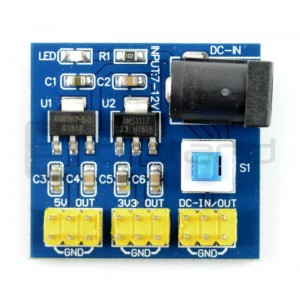
\includegraphics[width=0.5\textwidth]{inzynierku/img/zasilajacy.jpg}
\caption{\label{fig:modul_zasilajacy}Moduł zasilający 3,3V / 5V.}
\end{figure}

\subsection{Stabilizacja napięcia z baterii}
Do ustabilizowania napięcia ze źródła zasilania używana jest przetwornica. Przetwornica w porównaniu do stabilizatorów liniowych wydziela mniejsza ilość ciepła, a także pozwala na pracę z napięciem wejściowym mniejszym od napięcia wyjściowego. Użycie przetwornicy wymaka jednakże filtrację napięcia za pomocą kondensatorów. Zastosowanie tego elementu pozwala także na przetwarzanie wyższych natężeń prądu niż stabilizator. W projekcie przewidziane jest zasilanie bateryjne, jednakże silniki potrzebują napięcia 12V, które ma na celu dostarczyć chronić przed spadkami napięcia spowodowanym rozładowaniem źródła zasilania.
\begin{figure}[H]
\centering
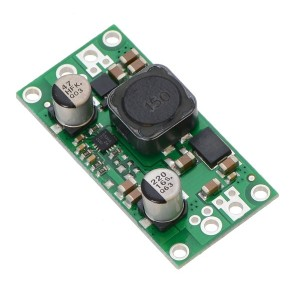
\includegraphics[width=0.5\textwidth]{inzynierku/img/przetwornica.jpg}
\caption{\label{fig:przetwornica_up_down}Pololu S18V20F12 - przetwornica step-up/down - 12V 2A.}
\end{figure}

\subsection{Płytka rozruchowa}
Płytką użytą w projekcie jest klon Arduino MEGA. Wybór tej płytki jest bezpośrednio powiązany z faktem, iż producenci często udostępniają biblioteki do obsługi czujników dla tego właśnie środowiska. Ze względu na liniowy charakter algorytmu, oraz niskie obciążenie procesora nie ma potrzeby wykorzystywania rozwiązań konkurencji, zawierających obsługę przerwań czy DMA. Użycie innego środowiska wiąże się z przepisaniem bibliotek. Płytka w użytej wersji zawiera:
\begin{itemize}
    \item 54 cyfrowych wejść/wyjść cyfrowych;
    \item w tym 15 można wykorzystać jako wyjścia PWM;
    \item 16 wejść analogowych;
    \item zegarowym o częstotliwości 16 MHz;
    \item 256 kB pamięci programu Flash;
    \item 8 kB pamięci operacyjnej SRAM;
    \item UART;
    \item I2C;
    \item SPI.
\end{itemize}
\begin{figure}[H]
\centering
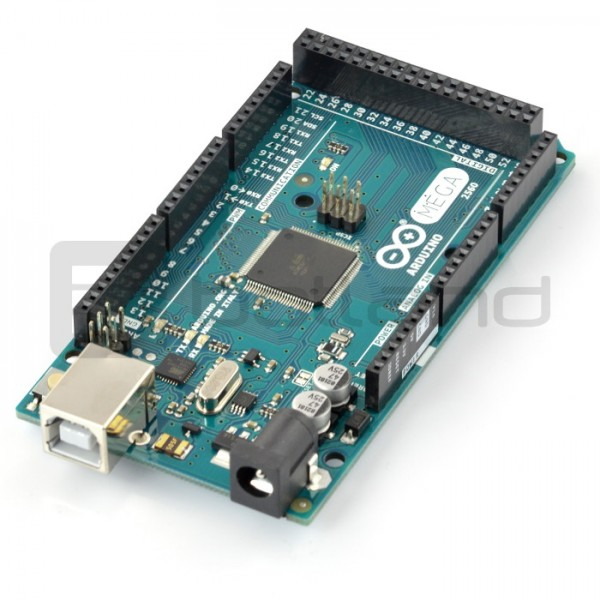
\includegraphics[width=0.5\textwidth]{inzynierku/img/arduino.jpg}
\caption{\label{fig:Arduino_MEGA}Płytka rozruchowa Arduino MEGA.}
\end{figure}

\section{Opis i schemat połączeń}
Podział zasilania zrobiony jest na płytce stykowej, natomiast sygnały podpięte są bezpośredni do płytki rozruchowej.
%\begin{figure}[H]
%\centering
%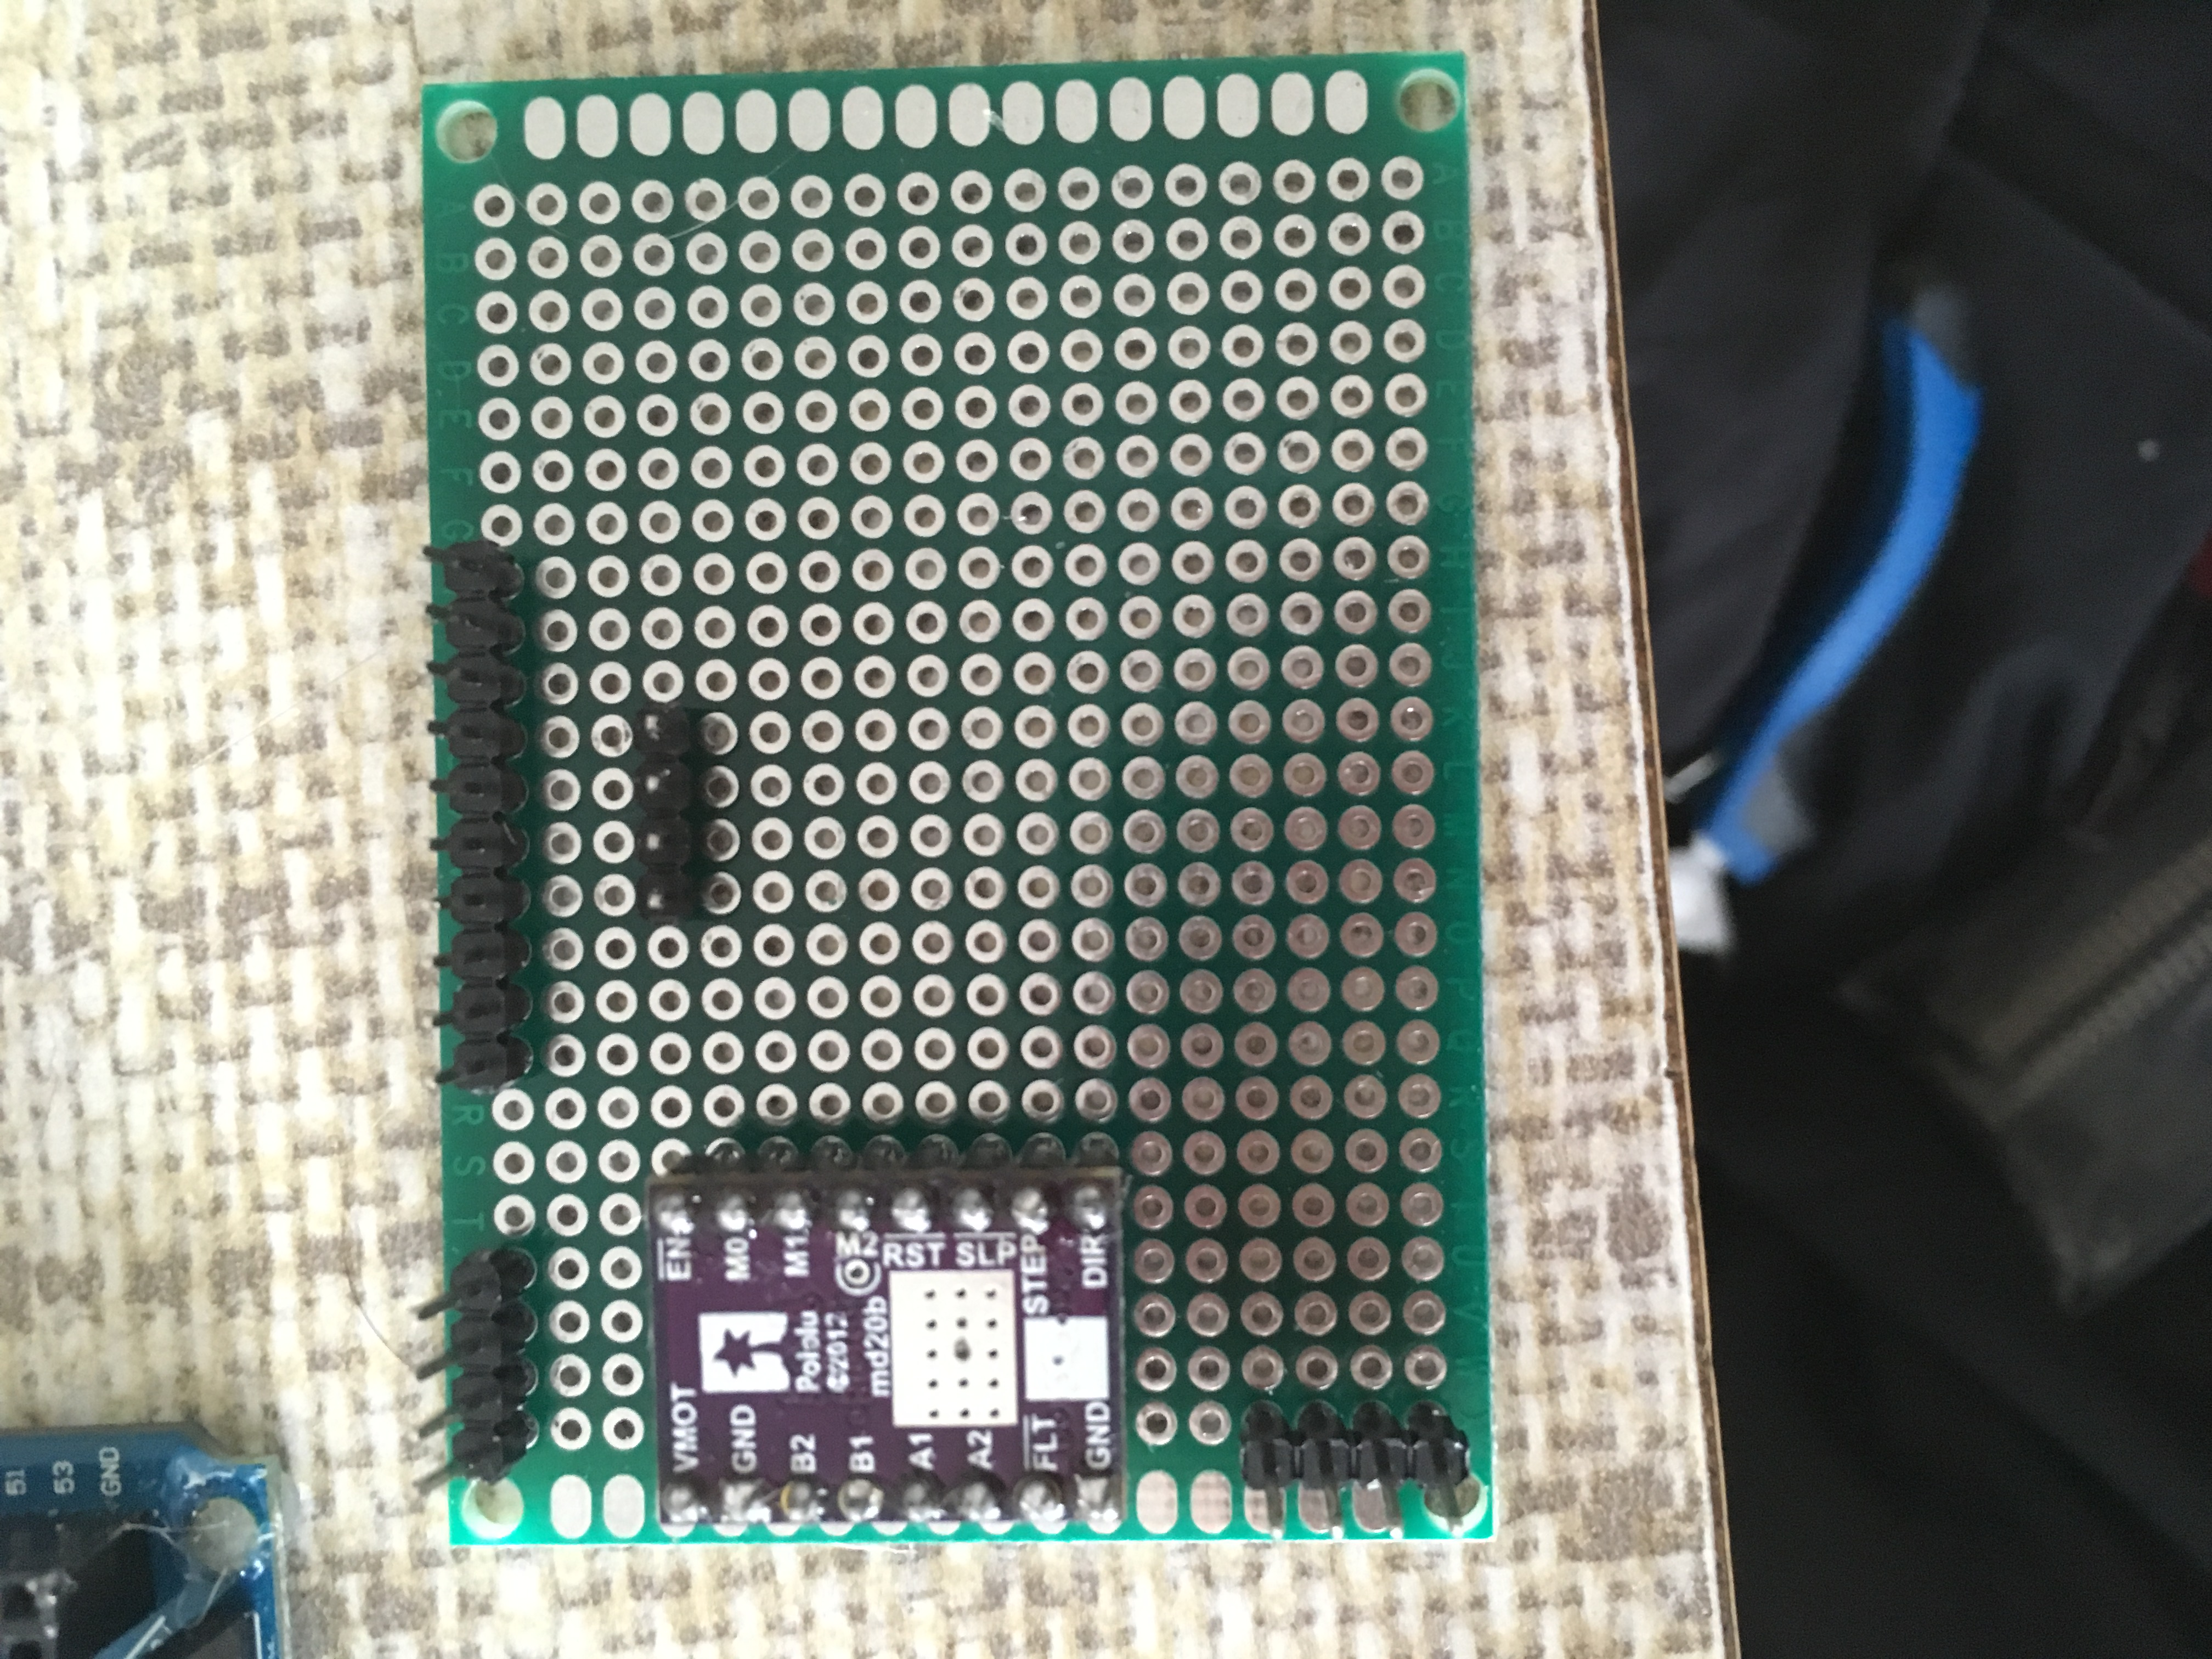
\includegraphics[width=0.5\textwidth]{inzynierku/img/plytka.jpg}
%\caption{\label{fig:plytka}Moduł podziału sygnałów i zasilania.}
%\end{figure}

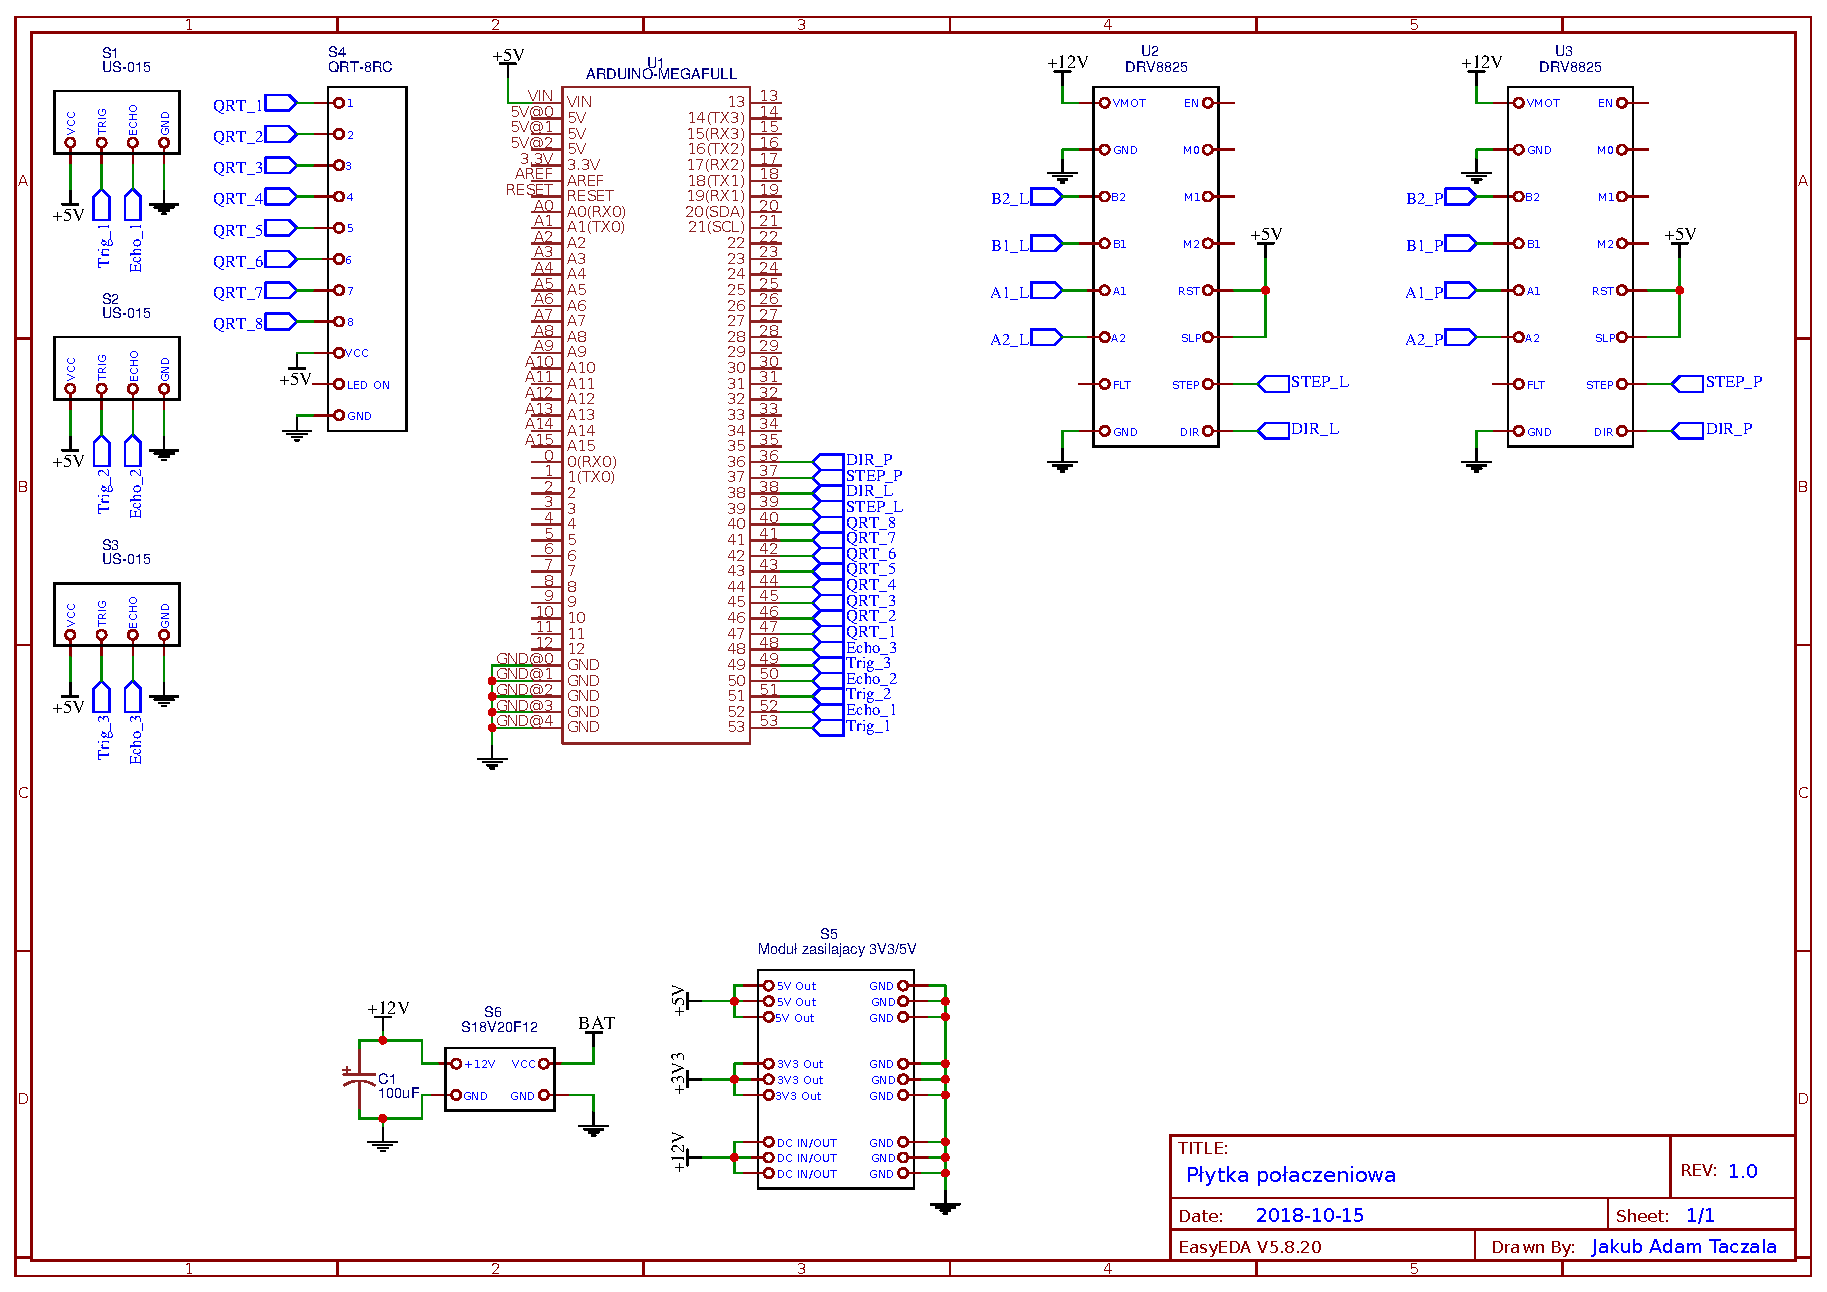
\includepdf{schematic.pdf}

\chapter{Problem podążania po wyznaczonej ścieżce}
\begin{figure}[H]
\centering
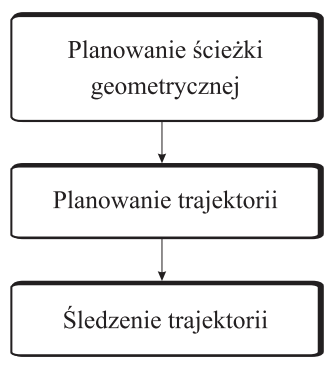
\includegraphics[width=0.5\textwidth]{inzynierku/img/planowanie.png}
\caption{\label{fig:planowanie}Planowanie ruchu \cite{planowanie_ruchu}.}
\end{figure}
Zadanie planowania ścieżki można podzielić na trzy etapy:
\begin{enumerate}
    \item Planowanie ścieżki geometrycznej -- wybór sposobu poruszania się robota, tj. czy platforma ma poruszać się do przodu czy też ma przyjąć rotację w jedna ze stron.
    \item Planowanie trajektorii -- określenie o ile kroków ma się poruszać w danym kierunku.
    \item Śledzenie trajektorii -- Na podstawie danych odbieranych przez czujniki określenie czy zadana trajektoria nie odbiega od zamierzonej ścieżki.
\end{enumerate}
Roboty mobilne o małej prędkości $V_{max}$ takie jak robot wykonany w projekcie, ze względu na niskie oddziaływanie sił bezwładności często są traktowane jako układy holonomiczne. \cite{planowanie_ruchu} W przypadku osiągania dużych prędkości przez robota należał oby uwzględnić poślizg kół, jednakże przez nagromadzenie wielu zmiennych wpływających wówczas na trajektorię, należy skorzystać z odpowiedzi otoczenia o położeniu układu.

W przypadku robota w układzie (2, 0) można skorzystać z metody halsowania znanej ze sposobu poruszania się łodzi żaglowych pod wiatr. Metoda ta pozwala na to by zawsze choć jeden czujnik znajdował się nad linią, jednocześnie upraszcza to sterowanie robotem jedynie do jazdy prawym bądź lewym kołem w przód.

W razie potrzeby porzucenia linii, najbezpieczniejszą metodą jest utrzymywanie robota w stałej odległości od przeszkody próbując ja w ten sposób ominąć przeszkodę i powrócić na linię. Jednakże ze względu na nieznajomość otoczenia należy uwzględnić sytuacje, w której to przeszkoda znajduje się np. w futrynie i po przebyciu określonej odległości zaprzestać kontynuacji zadania.

\section{Przyjęte ograniczenia robota oraz środowiska}
W ramach przedstawionego problemu przyjęto następujące uproszczenia:
\begin{enumerate}
    \item Robot jest jedynym obiektem przemieszczającym się w przestrzeni.
    \item Przestrzeń po której porusza się robot jest płaska.
    \item Przestrzeń po której porusza się robot jest gładka.
    \item Między kołami robota, a podłożem panuje idealna przyczepność.
    \item Podłoże jest białe, a ślad po którym porusza się robot wyznacza czarna linia.
    \item Pomieszczenie jest oświetlone przynajmniej na poziomie 300 luxów.
\end{enumerate}

\section{Ograniczenia konstrukcji robota}
\begin{enumerate}
    \item Koła porusza się z prędkością nie większą niż $100RPM$.
    \item Obiekt do ominięcia znajduje się na wysokości czujników ultradźwiękowych.
    \item Korytarz po którym porusza robot nie może być węższy niż 38cm.
    \item Przed wypuszczeniem robota na trasę należy przeprowadzić kalibrację czujników.
    \item Napięcie zasilania wynosi $3V-30V$.
\end{enumerate}